% This is the Amherst College LaTeX thesis template.
% See http://web.reed.edu/cis/help/latex.html for help. There are a
% great bunch of help pages there, with notes on
% getting started, bibtex, etc. Go there and read it if you're not
% already familiar with LaTeX.
%
% Any line that starts with a percent symbol is a comment.
% They won't show up in the document, and are useful for notes
% to yourself and explaining commands.
% Commenting also removes a line from the document;
% very handy for troubleshooting problems. -BTS

% As far as I know, this follows the requirements laid out in
% the 2002-2003 Senior Handbook. Ask a librarian to check the
% document before binding. -SN

%%
%% Preamble
%%
% \documentclass{<something>} must begin each LaTeX document
\documentclass[12pt,twoside]{amherstthesis}
% Packages are extensions to the basic LaTeX functions. Whatever you
% want to typeset, there is probably a package out there for it.
% Chemistry (chemtex), screenplays, you name it.
% Check out CTAN to see: http://www.ctan.org/
%%
\usepackage{graphicx,latexsym}
\usepackage{amsmath}
\usepackage{amssymb,amsthm}
\usepackage{longtable,booktabs,setspace}
\usepackage{chemarr} %% Useful for one reaction arrow, useless if you're not a chem major
\usepackage{rotating}

% Modified by CII
\usepackage[hyphens]{url}
\usepackage{hyperref}
\usepackage{lmodern}

% Added by CII (Thanks, Hadley!)
% Use ref for internal links
\renewcommand{\hyperref}[2][???]{\autoref{#1}}
\def\chapterautorefname{Chapter}
\def\sectionautorefname{Section}
\def\subsectionautorefname{Subsection}

\usepackage{caption}
\captionsetup{width=5in}

% \usepackage{times} % other fonts are available like times, bookman, charter, palatino

\title{My Comprehensive Evaluation}
\author{Kaitlyn E. Haase}
% The month and year that you submit your FINAL draft TO THE LIBRARY (May or December)
\date{February 2019}
\division{Statistics}
\advisor{Advisor A. Wagaman}
%If you have two advisors for some reason, you can use the following
%\altadvisor{Your Other Advisor}
%%% Remember to use the correct department!
\department{Mathematics and Statistics}
% if you're writing a thesis in an interdisciplinary major,
% uncomment the line below and change the text as appropriate.
% check the Senior Handbook if unsure.
%\thedivisionof{The Established Interdisciplinary Committee for}
% if you want the approval page to say "Approved for the Committee",
% uncomment the next line
%\approvedforthe{Committee}

% Below added by CII

%%% Copied from knitr
%% maxwidth is the original width if it's less than linewidth
%% otherwise use linewidth (to make sure the graphics do not exceed the margin)
\makeatletter
\def\maxwidth{ %
  \ifdim\Gin@nat@width>\linewidth
    \linewidth
  \else
    \Gin@nat@width
  \fi
}
\makeatother

\renewcommand{\contentsname}{Table of Contents}

\setlength{\parskip}{0pt}

\providecommand{\tightlist}{%
  \setlength{\itemsep}{0pt}\setlength{\parskip}{0pt}}

\Acknowledgements{
I want to thank my family.
}

\Dedication{

}

\Preface{

}

\Abstract{
In recent years, the amount of geographic data has increased immensely.
With new technology, the accuracy and complexity of data has also
improved. This has provoked statisticians to create techniques to best
analyze and draw conclusions from this new-found data. Earlier
techniques of spatial data were not equipped to handle the complexity
and amount of present data. This project first explores how and why we
analyze data based on geographic information. The project will then
focus on the CLARANS (Clustering Large Applications based on RANdomized
Search) algorithm, which is an extension of both the PAM (Partitioning
Around Medoids) and CLARAS (Clustering LARge Applications). Example data
will be used to demonstrate CLARANS, and the project will conclude by
testing how accurate CLARANS clustered the data.
}


%%
%% End Preamble
%%
%

\begin{document}

      \maketitle
  
  \frontmatter % this stuff will be roman-numbered
  \pagestyle{empty} % this removes page numbers from the frontmatter

      \begin{acknowledgements}
      I want to thank my family.
    \end{acknowledgements}
  
  
  % Add table of abbreviations?

      \hypersetup{linkcolor=black}
    \setcounter{tocdepth}{2}
    \tableofcontents
  
      \listoftables
  
      \listoffigures
  
      \begin{abstract}
      In recent years, the amount of geographic data has increased immensely.
      With new technology, the accuracy and complexity of data has also
      improved. This has provoked statisticians to create techniques to best
      analyze and draw conclusions from this new-found data. Earlier
      techniques of spatial data were not equipped to handle the complexity
      and amount of present data. This project first explores how and why we
      analyze data based on geographic information. The project will then
      focus on the CLARANS (Clustering Large Applications based on RANdomized
      Search) algorithm, which is an extension of both the PAM (Partitioning
      Around Medoids) and CLARAS (Clustering LARge Applications). Example data
      will be used to demonstrate CLARANS, and the project will conclude by
      testing how accurate CLARANS clustered the data.
    \end{abstract}
  
  
  \mainmatter % here the regular arabic numbering starts
  \pagestyle{fancyplain} % turns page numbering back on

  \onehalfspacing
  
  \chapter*{Introduction}\label{introduction}
  \addcontentsline{toc}{chapter}{Introduction}
  
  Data includes: latitude and longtitude, zip code, street address, etc.
  
  \section{Why Analyze Spatial Data?}\label{why-analyze-spatial-data}
  
  We want to analyze spatial data because there is so much of it
  available.
  
  \section{Big Picture Clustering
  Algorithms}\label{big-picture-clustering-algorithms}
  
  There are many clustering algorithms out there.
  
  \subsection{Classification
  vs.~Clustering}\label{classification-vs.clustering}
  
  Two categories of how to analyze spatial data include classification and
  clustering. Classification is BLANK Clustering is organizing a set of
  data items into groups so that items in the same group are similar to
  each other and different from those in other groups {[}Rec 1{]}.
  Clustering is helpful in finding patterns and similarities/differences
  between data points and groups; however it can be quite subjective, as
  we will discuss later on in the project.
  
  \hypertarget{rmd-basics}{\chapter{Spatial Clustering
  Methods}\label{rmd-basics}}
  
  There are many factors to consider when chosing a clustering algorithm,
  such as the application of the problem (what do you want to find out
  about this data?), quality vs speed trade off (size of data plays a
  role), characteristics of the data (i.e.~numeric distance measures),
  dimensionality (typically as dimension increases the time it takes to
  run the method increases and quality of the data clusters decrease), and
  outliers (some methods are very sensitive to outliers) {[}Rec 2{]}.
  
  \section{Types of Clustering: Partitioning and
  Hierarchical}\label{types-of-clustering-partitioning-and-hierarchical}
  
  There are many types of clustering algorithms, two of which are:
  partitioning and hierarchial.
  
  Hierarchial clustering organizes data items into a hierarchy with a
  sequence of nested partions or groupings {[}Rec 1, p.~405{]}. There is
  the bottom-up approach: There is also the top-down approach:
  
  Partitioning cluster methods divide a set of data items into a number of
  non-overlapping clusters. A data item is typically assigned to a cluster
  based on a proximity or dissimilarity measure {[}Rec 2, p.~405{]}.
  Partitioning clustering algorithms classifies the data into K groups by
  satisfying both that each group has at least one data point, and that
  each data point belongs to exactly one group. {[}Rec 5, p.~18{]}.
  
  \section{How to Create Clusters: K-Means vs
  K-Medoids}\label{how-to-create-clusters-k-means-vs-k-medoids}
  
  K-means algorithm and k-medoid algorithm are two examples of
  partitioning algorithms. They both ise iterative processes to find K
  clusters; however, they use different ways to represent these clusters.
  
  K-means algorithm represents its n observations in k groups, with the
  center of the groups being the mean/average observation.
  
  \textbf{Steps on p.~4, Rec 2 Also, it tries to minimize the objective
  function, steps on this page: }* Rec 5, p.~18
  
  Instead of taking the mean value of the objects in a cluster, the
  k-medoid method uses the most centrally located object in a cluster to
  be the cluster center {[}Rec 2{]}. This causes the method to be less
  sensitive to outliers, but also requires more time to run.
  
  \textbf{same steps as K-means except BLANK (p.~6 in Rec 2) }steps in Rec
  5, p.~19 for k-medoids
  
  \section{PAM}\label{pam}
  
  Partitioning Around Medoids (PAM) is a k-medoid method that iterates
  through all the k cluster centers and tries to replace the center with
  one of the other objects (n-k possibilities). {[}rec 2{]}. For a
  replacement to occur, the squared error function must decrease (if it
  does not decrease, there is no replacement). The algorithm eventually
  terminates with a local optimum.
  
  The total complexity of PAM in one iteration is **formula:
  O(k(n-k)\^{}2) (o= each non-medoid data point, k= \# of cluster centers,
  (n-k) objects to compare to, and (n-k) operations for calculating E).
  This makes for a costly computation when n is large. Works best for n=
  100, k=5.
  
  \section{CLARA}\label{clara}
  
  Because PAM does not scale well to large data sets, Clustering LARge
  Applications (CLARA) was developed to deal with larger data sets.
  
  CLARA is a sampling based method, meaning a sample of the data is used
  to represent the entire data set. Medoids are chosen from this sample
  data using PAM and then ``the average dissimilarity is computed using
  the whole dataset'' (**don't know what ``average dissimilarity'' means
  or how it is calculated). If a new set of medoids gives a lower
  dissimilarity than a previous best solution, then the best solution is
  replaced with a new set of medoids {[}Rec 2, p.~7{]}.
  
  \section{CLARANS (?)}\label{clarans}
  
  \chapter{Example}\label{typeset-equ}
  
  \section{Exploring the Data}\label{exploring-the-data}
  
  \section{Appplying CLARA}\label{appplying-clara}
  
  \section{Evaluation of CLARA}\label{evaluation-of-clara}
  
  \subsection{Model to Predict Cluster}\label{model-to-predict-cluster}
  
  \hypertarget{ref_labels}{\chapter{Tables, Graphics, References, and
  Labels}\label{ref_labels}}
  
  \section{Tables}\label{tables}
  
  In addition to the tables that can be automatically generated from a
  data frame in \textbf{R} that you saw in {[}R Markdown Basics{]} using
  the \texttt{kable} function, you can also create tables using
  \emph{pandoc}. (More information is available at
  \url{http://pandoc.org/README.html\#tables}.) This might be useful if
  you don't have values specifically stored in \textbf{R}, but you'd like
  to display them in table form. Below is an example. Pay careful
  attention to the alignment in the table and the use of the hyphens to
  create the rows and columns.
  
  \begin{longtable}[]{@{}ccc@{}}
  \caption{Correlation of Inheritance Factors for Parents and Child
  \label{tab:inher}}\tabularnewline
  \toprule
  \begin{minipage}[b]{0.29\columnwidth}\centering\strut
  Factors\strut
  \end{minipage} & \begin{minipage}[b]{0.47\columnwidth}\centering\strut
  Correlation between Parents \& Child\strut
  \end{minipage} & \begin{minipage}[b]{0.16\columnwidth}\centering\strut
  Inherited\strut
  \end{minipage}\tabularnewline
  \midrule
  \endfirsthead
  \toprule
  \begin{minipage}[b]{0.29\columnwidth}\centering\strut
  Factors\strut
  \end{minipage} & \begin{minipage}[b]{0.47\columnwidth}\centering\strut
  Correlation between Parents \& Child\strut
  \end{minipage} & \begin{minipage}[b]{0.16\columnwidth}\centering\strut
  Inherited\strut
  \end{minipage}\tabularnewline
  \midrule
  \endhead
  \begin{minipage}[t]{0.29\columnwidth}\centering\strut
  Education\strut
  \end{minipage} & \begin{minipage}[t]{0.47\columnwidth}\centering\strut
  -0.49\strut
  \end{minipage} & \begin{minipage}[t]{0.16\columnwidth}\centering\strut
  Yes\strut
  \end{minipage}\tabularnewline
  \begin{minipage}[t]{0.29\columnwidth}\centering\strut
  Socio-Economic Status\strut
  \end{minipage} & \begin{minipage}[t]{0.47\columnwidth}\centering\strut
  0.28\strut
  \end{minipage} & \begin{minipage}[t]{0.16\columnwidth}\centering\strut
  Slight\strut
  \end{minipage}\tabularnewline
  \begin{minipage}[t]{0.29\columnwidth}\centering\strut
  Income\strut
  \end{minipage} & \begin{minipage}[t]{0.47\columnwidth}\centering\strut
  0.08\strut
  \end{minipage} & \begin{minipage}[t]{0.16\columnwidth}\centering\strut
  No\strut
  \end{minipage}\tabularnewline
  \begin{minipage}[t]{0.29\columnwidth}\centering\strut
  Family Size\strut
  \end{minipage} & \begin{minipage}[t]{0.47\columnwidth}\centering\strut
  0.18\strut
  \end{minipage} & \begin{minipage}[t]{0.16\columnwidth}\centering\strut
  Slight\strut
  \end{minipage}\tabularnewline
  \begin{minipage}[t]{0.29\columnwidth}\centering\strut
  Occupational Prestige\strut
  \end{minipage} & \begin{minipage}[t]{0.47\columnwidth}\centering\strut
  0.21\strut
  \end{minipage} & \begin{minipage}[t]{0.16\columnwidth}\centering\strut
  Slight\strut
  \end{minipage}\tabularnewline
  \bottomrule
  \end{longtable}
  
  We can also create a link to the table by doing the following:
  \autoref{tab:inher}. If you go back to {[}Loading and exploring data{]}
  and look at the \texttt{kable} function code, you'll see that I added in
  a similar \texttt{\textbackslash{}\textbackslash{}label} to be able to
  reference that table later. (The extra backslash there is a way that
  \emph{Markdown} interfaces with \LaTeX.) We can create a reference to
  the max delays table: \autoref{tab:max_delay}.
  
  The addition of the \texttt{\textbackslash{}label\{\}} option to the end
  of the table caption allows us to then use the \LaTeX~\texttt{autoref}
  function to produce the link. The \texttt{ref} function in \textbf{R}
  allows for tables and figures to be referenced in the document easily
  without having to directly use the \texttt{autoref} function. It will
  automatically add ``Table'' before your number if you add the ``tab:''
  prefix to your label. Note that this reference could appear anywhere
  throughout the document.
  
  \clearpage
  
  \section{Figures}\label{figures}
  
  If your thesis has a lot of figures, \emph{R Markdown} might behave
  better for you than that other word processor. One perk is that it will
  automatically number the figures accordingly in each chapter. You'll
  also be able to create a label for each figure, add a caption, and then
  reference the figure in a way similar to what we saw with tables
  earlier. If you label your figures, you can move the figures around and
  \emph{R Markdown} will automatically adjust the numbering for you. No
  need for you to remember! So that you don't have to get too far into
  \LaTeX~to do this, a couple \textbf{R} functions have been created for
  you to assist. You'll see their use below.
  
  In the \textbf{R} chunk below, we will load in a picture stored as
  \texttt{amherst.png} in our main directory. We then give it the caption
  of ``Amherst logo'', the label of ``amherst'', and specify that this is
  a figure. Note again the use of the \texttt{results\ =\ "asis"}
  specification to automatically include and compile the \LaTeX~code.
  
  \begin{Shaded}
  \begin{Highlighting}[]
  \KeywordTok{label}\NormalTok{(}\DataTypeTok{path =} \StringTok{"figure/amherst.png"}\NormalTok{, }\DataTypeTok{caption =} \StringTok{"Amherst logo"}\NormalTok{, }
        \DataTypeTok{label =} \StringTok{"amherst"}\NormalTok{, }\DataTypeTok{type =} \StringTok{"figure"}\NormalTok{)}
  \end{Highlighting}
  \end{Shaded}
  
  \begin{figure}[htbp]
  \centering
  
\includegraphics[scale = 1,angle = 0]{figure/amherst.png}
  \caption[Amherst logo]{\normalsize{Amherst logo}}
  \label{fig:amherst}
  \end{figure}
  
  Here is a reference to the Amherst logo: \autoref{fig:amherst}. Note the
  use of the inline \textbf{R} code here. By default ``figure'' is
  specified as the type. For clarity, we could have also added the
  \texttt{label} and \texttt{type} to the parameter specifications and
  this would give us the same result: \autoref{fig:amherst}.
  
  \clearpage 
  
  Below we will investigate how to save the output of an \textbf{R} plot
  and label it in a way similar to that done above. Recall the
  \texttt{flights} dataset from \protect\hyperlink{rmd-basics}{}. (Note
  that we've shown a different way to reference a section or chapter
  here.) We will next explore a bar graph with the mean flight departure
  delays by airline from Portland for 2014. Note also the use of the
  \texttt{scale} parameter which is discussed on the next page.
  
  \begin{Shaded}
  \begin{Highlighting}[]
  \NormalTok{delay_airline <-}\StringTok{ }\NormalTok{flights }\OperatorTok\StringTok{ }\KeywordTok{group_by}\NormalTok{(carrier) }\OperatorTok
  \StringTok{  }\KeywordTok{summarize}\NormalTok{(}\DataTypeTok{mean_dep_delay =} \KeywordTok{mean}\NormalTok{(dep_delay)) }\OperatorTok
  \StringTok{  }\KeywordTok{ggplot}\NormalTok{(}\KeywordTok{aes}\NormalTok{(}\DataTypeTok{x =}\NormalTok{ carrier, }\DataTypeTok{y =}\NormalTok{ mean_dep_delay)) }\OperatorTok{+}
  \StringTok{  }\KeywordTok{geom_bar}\NormalTok{(}\DataTypeTok{position =} \StringTok{"identity"}\NormalTok{, }\DataTypeTok{stat =} \StringTok{"identity"}\NormalTok{, }\DataTypeTok{fill =} \StringTok{"red"}\NormalTok{)}
  \KeywordTok{ggsave}\NormalTok{(}\StringTok{"figure/delays.png"}\NormalTok{, }\DataTypeTok{plot =}\NormalTok{ delay_airline, }
         \DataTypeTok{width =} \DecValTok{5}\NormalTok{, }\DataTypeTok{height =} \DecValTok{3}\NormalTok{)}
  \end{Highlighting}
  \end{Shaded}
  
  \begin{Shaded}
  \begin{Highlighting}[]
  \KeywordTok{label}\NormalTok{(}\DataTypeTok{path =} \StringTok{"figure/delays.png"}\NormalTok{, }
        \DataTypeTok{caption =} \StringTok{"Mean Delays by Airline"}\NormalTok{, }
        \DataTypeTok{label =} \StringTok{"delays"}\NormalTok{, }\DataTypeTok{type =} \StringTok{"figure"}\NormalTok{,}
        \DataTypeTok{scale =} \FloatTok{0.3}\NormalTok{)}
  \end{Highlighting}
  \end{Shaded}
  
  \begin{figure}[htbp]
  \centering
  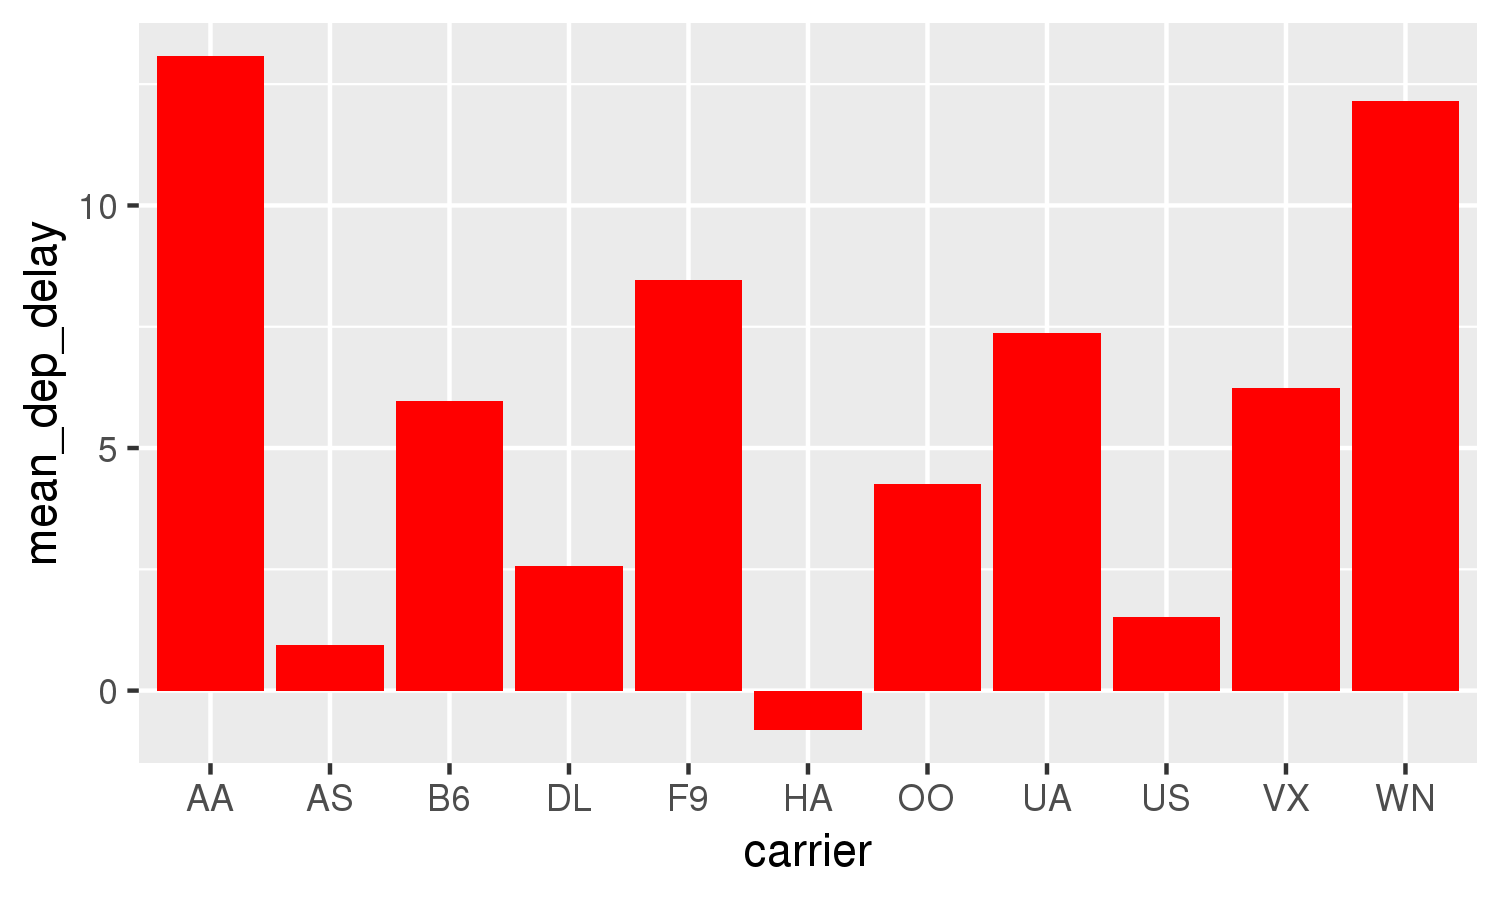
\includegraphics[scale = 0.3,angle = 0]{figure/delays.png}
  \caption[Mean Delays by Airline]{\normalsize{Mean Delays by Airline}}
  \label{fig:delays}
  \end{figure}
  
  A table linking these carrier codes to airline names is available at
  \url{https://github.com/ismayc/pnwflights14/blob/master/data/airlines.csv}.
  
  \clearpage
  
  Next, we will explore the use of the \texttt{scale} parameter which can
  be used to shrink or expand an image. Here we use the mathematical graph
  stored in the ``subdivision.pdf'' file. Note that we didn't specify the
  \texttt{caption\ =} or \texttt{label\ =} here, but we could have.
  
  \begin{Shaded}
  \begin{Highlighting}[]
  \KeywordTok{label}\NormalTok{(}\StringTok{"figure/subdivision.pdf"}\NormalTok{, }\StringTok{"Subdiv. graph"}\NormalTok{, }\StringTok{"subd"}\NormalTok{, }
        \DataTypeTok{scale =} \FloatTok{0.75}\NormalTok{)}
  \end{Highlighting}
  \end{Shaded}
  
  \begin{figure}[htbp]
  \centering
  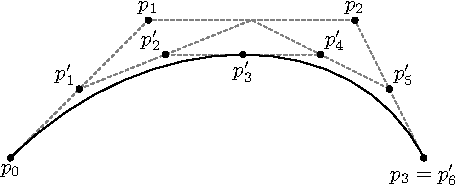
\includegraphics[scale = 0.75,angle = 0]{figure/subdivision.pdf}
  \caption[Subdiv. graph]{\normalsize{Subdiv. graph}}
  \label{fig:subd}
  \end{figure}
  
  Here is a reference to this image: \autoref{fig:subd}. (Move this around
  throughout the document as you wish.)
  
  \subsubsection{More Figure Stuff}\label{more-figure-stuff}
  
  Lastly, we will explore how to rotate figures using the \texttt{angle}
  parameter.
  
  \begin{Shaded}
  \begin{Highlighting}[]
  \KeywordTok{label}\NormalTok{(}\StringTok{"figure/subdivision.pdf"}\NormalTok{, }
        \StringTok{"A Larger Figure, Flipped Upside Down"}\NormalTok{, }
        \DataTypeTok{scale =} \FloatTok{1.5}\NormalTok{,}
        \DataTypeTok{angle =} \DecValTok{180}\NormalTok{,}
        \DataTypeTok{label =} \StringTok{"subd2"}\NormalTok{)}
  \end{Highlighting}
  \end{Shaded}
  
  \begin{figure}[htbp]
  \centering
  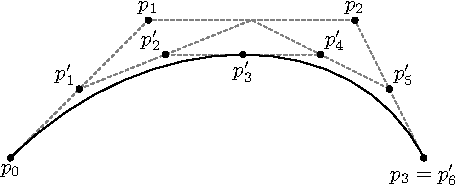
\includegraphics[scale = 1.5,angle = 180]{figure/subdivision.pdf}
  \caption[A Larger Figure, Flipped Upside Down]{\normalsize{A Larger Figure, Flipped Upside Down}}
  \label{fig:subd2}
  \end{figure}
  
  As another example, here is a reference to this figure:
  \autoref{fig:subd2}.
  
  \subsubsection{Common Modifications}\label{common-modifications}
  
  The following figure features the more popular changes thesis students
  want to their figures. We can add math to the caption that displays
  below the picture, specify the size of our caption to display below the
  figure (list of sizes available at this
  \href{http://www.emerson.emory.edu/services/latex/latex_169.html\#SEC169}{link}),
  and also specify that a different caption \texttt{alt.cap} be what
  appears in the Table of Figures for this figure.
  
  If you'd like to make further tweaks to figures, you might need to
  invoke some \LaTeX~code.
  
  \begin{Shaded}
  \begin{Highlighting}[]
  \KeywordTok{label}\NormalTok{(}\StringTok{"figure/subdivision.pdf"}\NormalTok{, }
        \DataTypeTok{caption =} \StringTok{"Subdivision of arc segments"}\NormalTok{,}
        \DataTypeTok{alt.cap =} \StringTok{"You can see that $p_3 = p_6^}\CharTok{\textbackslash{}\textbackslash{}}\StringTok{prime$"}\NormalTok{,}
        \DataTypeTok{cap.size =} \StringTok{"footnotesize"}\NormalTok{,}
        \DataTypeTok{label =} \StringTok{"subd3"}\NormalTok{)}
  \end{Highlighting}
  \end{Shaded}
  
  \begin{figure}[htbp]
  \centering
  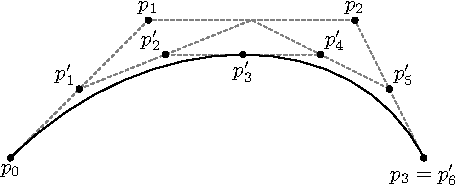
\includegraphics[scale = 1,angle = 0]{figure/subdivision.pdf}
  \caption[Subdivision of arc segments]{\footnotesize{You can see that $p_3 = p_6^\prime$}}
  \label{fig:subd3}
  \end{figure}
  
  \section{Footnotes and Endnotes}\label{footnotes-and-endnotes}
  
  You might want to footnote something.\footnote{footnote text} The
  footnote will be in a smaller font and placed appropriately. Endnotes
  work in much the same way.
  
  \section{Bibliographies}\label{bibliographies}
  
  Of course you will need to cite things, and you will probably accumulate
  an armful of sources. There are a variety of tools available for
  creating a bibliography database (stored with the .bib extension). In
  addition to BibTeX suggested below, you may want to consider using the
  free and easy-to-use tool called Zotero.
  
  \emph{R Markdown} uses \emph{pandoc} (\url{http://pandoc.org/}) to build
  its bibliographies. One nice caveat of this is that you won't have to do
  a second compile to load in references as standard \LaTeX~requires. To
  cite references in your thesis (after creating your bibliography
  database), place the reference name inside square brackets and precede
  it by the ``at'' symbol. For example, here's a reference to a book about
  worrying: (Molina \& Borkovec, 1994). This \texttt{Molina1994} entry
  appears in a file called \texttt{thesis.bib} in the \texttt{bib} folder.
  This bibliography database file was created by a program called BibTeX.
  You can call this file something else if you like (look at the YAML
  header in the main .Rmd file) and, by default, is to placed in the
  \texttt{bib} folder.
  
  For more information about BibTeX and bibliographies, see Reed College's
  CUS site (\url{http://web.reed.edu/cis/help/latex/index.html})\footnote{Reed~College
    (2007)}. There are three pages on this topic: \emph{bibtex} (which
  talks about using BibTeX, at
  \url{http://web.reed.edu/cis/help/latex/bibtex.html}),
  \emph{bibtexstyles} (about how to find and use the bibliography style
  that best suits your needs, at
  \url{http://web.reed.edu/cis/help/latex/bibtexstyles.html}) and
  \emph{bibman} (which covers how to make and maintain a bibliography by
  hand, without BibTeX, at
  \url{http://web.reed.edu/cis/help/latex/bibman.html}). The last page
  will not be useful unless you have only a few sources.
  
  If you look at the YAML header at the top of the main .Rmd file you can
  see that we can specify the style of the bibliography by referencing the
  appropriate csl file. You can download a variety of different style
  files at \url{https://www.zotero.org/styles}. Make sure to download the
  file into the csl folder.
  
  \paragraph{Tips for Bibliographies}\label{tips-for-bibliographies}
  
  \begin{itemize}
  \tightlist
  \item
    Like with thesis formatting, the sooner you start compiling your
    bibliography for something as large as thesis, the better. Typing in
    source after source is mind-numbing enough; do you really want to do
    it for hours on end in late April? Think of it as procrastination.
  \item
    The cite key (a citation's label) needs to be unique from the other
    entries.
  \item
    When you have more than one author or editor, you need to separate
    each author's name by the word ``and'' e.g.
    \texttt{Author\ =\ \{Noble,\ Sam\ and\ Youngberg,\ Jessica\},}.
  \item
    Bibliographies made using BibTeX (whether manually or using a manager)
    accept \LaTeX~markup, so you can italicize and add symbols as
    necessary.
  \item
    To force capitalization in an article title or where all lowercase is
    generally used, bracket the capital letter in curly braces.
  \end{itemize}
  
  \chapter*{Conclusion}\label{conclusion}
  \addcontentsline{toc}{chapter}{Conclusion}
  
  \setcounter{chapter}{4} \setcounter{section}{0}
  
  If we don't want Conclusion to have a chapter number next to it, we can
  add the \texttt{\{.unnumbered\}} attribute. This has an unintended
  consequence of the sections being labeled as 3.6 for example though
  instead of 4.1. The \LaTeX~commands immediately following the Conclusion
  declaration get things back on track.
  
  \subsubsection{More info}\label{more-info}
  
  And here's some other random info: the first paragraph after a chapter
  title or section head \emph{shouldn't be} indented, because indents are
  to tell the reader that you're starting a new paragraph. Since that's
  obvious after a chapter or section title, proper typesetting doesn't add
  an indent there.
  
  \appendix
  
  \singlespacing
  
  \chapter{The First Appendix}\label{the-first-appendix}
  
  This first appendix includes all of the R chunks of code that were
  hidden throughout the document (using the \texttt{include\ =\ FALSE}
  chunk tag) to help with readibility and/or setup.
  
  \subsubsection{In the main Rmd file:}\label{in-the-main-rmd-file}
  
  \begin{Shaded}
  \begin{Highlighting}[]
  \CommentTok{# This chunk ensures that the acstats package is}
  \CommentTok{# installed and loaded. This acstats package includes}
  \CommentTok{# the template files for the thesis and also two functions}
  \CommentTok{# used for labeling and referencing}
  \ControlFlowTok{if}\NormalTok{(}\OperatorTok{!}\KeywordTok{require}\NormalTok{(devtools))}
    \KeywordTok{install.packages}\NormalTok{(}\StringTok{"devtools"}\NormalTok{, }\DataTypeTok{repos =} \StringTok{"http://cran.rstudio.com"}\NormalTok{)}
  \ControlFlowTok{if}\NormalTok{(}\OperatorTok{!}\KeywordTok{require}\NormalTok{(acstats))\{}
    \KeywordTok{library}\NormalTok{(devtools)}
  \NormalTok{  devtools}\OperatorTok{::}\KeywordTok{install_github}\NormalTok{(}\StringTok{"Amherst-Statistics/acstats"}\NormalTok{)}
  \NormalTok{\}}
  \KeywordTok{library}\NormalTok{(acstats)}
  \end{Highlighting}
  \end{Shaded}
  
  \subsubsection{\texorpdfstring{In
  \protect\hyperlink{ref_labels}{}:}{In :}}\label{in}
  
  \begin{Shaded}
  \begin{Highlighting}[]
  \CommentTok{# This chunk ensures that the acstats package is}
  \CommentTok{# installed and loaded. This acstats package includes}
  \CommentTok{# the template files for the thesis and also two functions}
  \CommentTok{# used for labeling and referencing}
  \ControlFlowTok{if}\NormalTok{(}\OperatorTok{!}\KeywordTok{require}\NormalTok{(devtools))}
    \KeywordTok{install.packages}\NormalTok{(}\StringTok{"devtools"}\NormalTok{, }\DataTypeTok{repos =} \StringTok{"http://cran.rstudio.com"}\NormalTok{)}
  \ControlFlowTok{if}\NormalTok{(}\OperatorTok{!}\KeywordTok{require}\NormalTok{(dplyr))}
      \KeywordTok{install.packages}\NormalTok{(}\StringTok{"dplyr"}\NormalTok{, }\DataTypeTok{repos =} \StringTok{"http://cran.rstudio.com"}\NormalTok{)}
  \ControlFlowTok{if}\NormalTok{(}\OperatorTok{!}\KeywordTok{require}\NormalTok{(ggplot2))}
      \KeywordTok{install.packages}\NormalTok{(}\StringTok{"ggplot2"}\NormalTok{, }\DataTypeTok{repos =} \StringTok{"http://cran.rstudio.com"}\NormalTok{)}
  \ControlFlowTok{if}\NormalTok{(}\OperatorTok{!}\KeywordTok{require}\NormalTok{(acstats))\{}
    \KeywordTok{library}\NormalTok{(devtools)}
  \NormalTok{  devtools}\OperatorTok{::}\KeywordTok{install_github}\NormalTok{(}\StringTok{"Amherst-Statistics/acstats"}\NormalTok{)}
  \NormalTok{  \}}
  \KeywordTok{library}\NormalTok{(acstats)}
  \NormalTok{flights <-}\StringTok{ }\KeywordTok{read.csv}\NormalTok{(}\StringTok{"data/flights.csv"}\NormalTok{)}
  \end{Highlighting}
  \end{Shaded}
  
  \chapter{The Second Appendix, for
  Fun}\label{the-second-appendix-for-fun}
  
  \backmatter
  
  \chapter{References}\label{references}
  
  \noindent
  
  \setlength{\parindent}{-0.20in} \setlength{\leftskip}{0.20in}
  \setlength{\parskip}{8pt}
  
  \hypertarget{refs}{}
  \hypertarget{ref-angel2000}{}
  Angel, E. (2000). \emph{Interactive computer graphics : A top-down
  approach with opengl}. Boston, MA: Addison Wesley Longman.
  
  \hypertarget{ref-angel2001}{}
  Angel, E. (2001a). \emph{Batch-file computer graphics : A bottom-up
  approach with quicktime}. Boston, MA: Wesley Addison Longman.
  
  \hypertarget{ref-angel2002a}{}
  Angel, E. (2001b). \emph{Test second book by angel}. Boston, MA: Wesley
  Addison Longman.
  
  \hypertarget{ref-Molina1994}{}
  Molina, S. T., \& Borkovec, T. D. (1994). The Penn State worry
  questionnaire: Psychometric properties and associated characteristics.
  In G. C. L. Davey \& F. Tallis (Eds.), \emph{Worrying: Perspectives on
  theory, assessment and treatment} (pp. 265--283). New York: Wiley.
  
  \hypertarget{ref-reedweb2007}{}
  Reed~College. (2007, March). LaTeX your document. Retrieved from
  \url{http://web.reed.edu/cis/help/LaTeX/index.html}


  % Index?

\end{document}

